\addcontentsline{toc}{part}{Day 2: Advanced Kuali Enterprise Workflow}
\part*{Day 2\\
Advanced Kuali Enterprise Workflow}
\addcontentsline{toc}{section}{Exercise 3: Split Node}
{\setlength{\baselineskip}%
  {0.0\baselineskip}
  \section*{\flushright Exercise 3\\
  Complex Routing Patterns}
  \hrulefill \par}

\addcontentsline{toc}{subsection}{Description}
\subsection*{Description}
This exercise is going to build on another exercise taken from the
Basic Kuali Rice Training, and bring it all together as one complete
exercise. We are going to create a new type of product for sale that
is exactly like the previous. 

We are going to use an \emph{ImportedBookDocument} to demonstrate
capabilities for \emph{Complex Role-based Routing}, \emph{Complex
  Split Nodes}, \emph{Custom Document Type Statuses}, and 

\addcontentsline{toc}{subsection}{Goals}
\subsection*{Goals}
\begin{itemize}
\item create a split node based on the contents of a document
\item route to a responsibility based upon a role that is determined
  by a user's department
\item add a custom status to a document which will reveal more detail
  about routing
\item learn how to make a customized action list
\end{itemize}

\addcontentsline{toc}{subsection}{1 Inherited Routing}
\subsection*{1 Inherited Routing}
We will reuse the existing exercise information for our routing. We
will first need to create a new \textbf{ImportedBookOrderDocument} to
handle books imported from outside the US.

\subsubsection*{1.1 Create a new
  train.bookstore.document.ImportedBookOrderDocument}
Create a new class called \textbf{ImportedBookOrderDocument} in the
\textbf{train.bookstore.document} package. It will inherit from the
\textbf{train.bookstore.document.BookOrderDocument}

\subsubsection*{1.2 Create a new ImportedBookOrderDocument Workflow
  Doctype}
\begin{lstlisting}[numbers=left,language=xml,basicstyle=\scriptsize,backgroundcolor=\color{ubergray},caption={New
  ImportedBookOrderDocumentType},frame=single,breaklines=true]
<?xml version='1.0' encoding='UTF-8'?> 
<data xmlns="ns:workflow" xmlns:fo="http://www.w3.org/1999/XSL/Format" xmlns:xsi="http://www.w3.org/2001/XMLSchema-instance" xsi:schemaLocation="ns:workflow resource:WorkflowData">
  <documentTypes xmlns="ns:workflow/DocumentType" xsi:schemaLocation="ns:workflow/DocumentType resource:DocumentType">
    <documentType>
      <name>ImportedBookOrderDocumentType</name>
      <parent>BookOrderDocumentType</parent>
      <label>Imported Book Order</label>
    </documentType>
  </documentTypes>
</data>
\end{lstlisting}

\subsubsection*{1.3 Ingest the New Document Type}
\begin{enumerate}
  \item Start the Training Application
  \item Login as the \textbf{admin} user
  \item Select the \textbf{Administration} tab
  \item Locate \textbf{XML Ingester} under the \textbf{Workflow}
    Channel
  \item Ingest the document type here
\end{enumerate}

\subsubsection*{1.4 Create a new ImportedBookOrderDocument Workflow
  Doctype}
The application should already be started. You can try and test it
out. The behavior should be the same for the
\textbf{ImportedBookOrderDocument} as for the
\textbf{BookOrderDocument} to \emph{Fiscal Approval}.

\subsubsection*{1.5 Create a new ImportedBookOrderDocument.xml
  DataDictionary Entry}
We also need to create a DataDictionary entry for the new
\textbf{ImportedBookOrderDocument}.
\begin{enumerate}
  \item Edit
    \textbf{src/main/resources/train/bookstore/document/datadictionary/ImportedBookOrderDocument.xml}
  \item Create a bean that inherits from the
    \textbf{BookOrderDocument}
\begin{lstlisting}[numbers=left,language=xml,basicstyle=\scriptsize,backgroundcolor=\color{ubergray},caption={ImportBookOrderDocument.xml},frame=single,breaklines=true]
  <bean id="ImportedBookOrderDocument-parentBean" abstract="true" parent="BookOrderDocument-parentBean">
	<property name="documentTypeName" value="ImportedBookOrderDocumentType"/>
	<property name="documentClass"
    value="train.bookstore.document.ImportedBookOrderDocument"/>
  \end{lstlisting}
\end{enumerate}

The final data dictionary entry looks like:
\begin{lstlisting}[numbers=left,language=xml,basicstyle=\scriptsize,backgroundcolor=\color{ubergray},caption={ImportBookOrderDocument.xml},frame=single,breaklines=true]
<?xml version="1.0" encoding="UTF-8"?>
<beans xmlns="http://www.springframework.org/schema/beans" xmlns:xsi="http://www.w3.org/2001/XMLSchema-instance" xmlns:p="http://www.springframework.org/schema/p" xmlns:dd="http://rice.kuali.org/dd" xsi:schemaLocation="http://www.springframework.org/schema/beans     	http://www.springframework.org/schema/beans/spring-beans-2.0.xsd     	http://rice.kuali.org/dd     	http://rice.kuali.org/dd/dd.xsd">


  <bean id="ImportedBookOrderDocument" parent="ImportedBookOrderDocument-parentBean"/>

  <bean id="ImportedBookOrderDocument-parentBean" abstract="true" parent="BookOrderDocument-parentBean">
	<property name="documentTypeName" value="ImportedBookOrderDocumentType"/>
	<property name="documentClass"
    value="train.bookstore.document.ImportedBookOrderDocument"/>
</beans>
\end{lstlisting}


\addcontentsline{toc}{subsection}{2 Complex Role-Based Routing}
\subsection*{2 Role-Based Routing}
For imported books, they will need to first go through Customs.

\subsection*{2.1 Create the Customs Derived Role}
To do this we will need a KIM Type. We will make the KIM Type first
and then the role.
\subsubsection*{2.1.1 Stub a CustomsDerivedRoleTypeServiceImpl class}
Add the following class to \textbf{train.bookstore.identity.service.impl}
\begin{lstlisting}[numbers=left,language=java,basicstyle=\scriptsize,backgroundcolor=\color{ubergray},caption={Stubbed
  CustomsDerivedRoleTypeServiceImpl.java},frame=single,breaklines=true]
public class CustomsDerivedRoleTypeServiceImpl extends KimDerivedRoleTypeServiceBase {
    /**
     * 
     * @see org.kuali.rice.kim.service.support.impl.KimRoleTypeServiceBase#getPrincipalIdsFromApplicationRole(java.lang.String, java.lang.String, org.kuali.rice.kim.bo.types.dto.AttributeSet)
     */
    @Override
    public List<RoleMembershipInfo> getRoleMembersFromApplicationRole(String namespaceCode, String roleName, AttributeSet qualification) {
        final List<RoleMembershipInfo> members = new ArrayList<RoleMembershipInfo>();
        return members
    }
}
\end{lstlisting}

Currently, this will return just about anyone. What we intend to do is
return only add a user to the Customs Role when a person is found in
the \textbf{CUSTOMS} department. This means we will need to make use
of KIM and the \textbf{PersonService} to do this. 

\subsubsection*{2.1.2 Inject the PersonService}
\begin{lstlisting}[numbers=left,language=java,basicstyle=\scriptsize,backgroundcolor=\color{ubergray},caption={Stubbed
    CustomsDerivedRoleTypeServiceImpl.java},frame=single,breaklines=true]

    private PersonService personService;

    public void setPersonService(final PersonService personService) {
        this.personService = personService;
    }

    protected PersonService getPersonService() {
        return personService;
    }
\end{lstlisting}

\subsubsection*{2.1.2 Finish Implementing
  getRoleMembersFromApplicationRole}
So far, this is what we have:
\begin{lstlisting}[numbers=left,language=java,basicstyle=\scriptsize,backgroundcolor=\color{ubergray},caption={Stubbed
  customsDerivedRoleTypeServiceImpl.java},frame=single,breaklines=true]
    public List<RoleMembershipInfo> getRoleMembersFromApplicationRole(String namespaceCode, String roleName, AttributeSet qualification) {
        final List<RoleMembershipInfo> members = new ArrayList<RoleMembershipInfo>();
        return members;
    }
\end{lstlisting}

What we want to do is implement this to use the \textbf{findPeople()}
method in \textbf{PersonService}
to lookup all \textbf{Person} instances where
\textbf{primaryDepartmentCode} is \emph{CUSTOMS}.

Once we have those \textbf{Person} instances, we are going to need to
create \textbf{RoleMembershipInfo} instances from those and add them
to our list of members. To do that you want to use something like:

\begin{lstlisting}[numbers=left,language=java,basicstyle=\scriptsize,backgroundcolor=\color{ubergray},caption={New
  RoleMembershipInfo snippet},frame=single,breaklines=true]
final RoleMembershipInfo member = new RoleMembershipInfo(null,null,person.getPrincipalId(),Role.PRINCIPAL_MEMBER_TYPE,null) 
\end{lstlisting}

\subsubsection*{2.1.2 Configure the CustomsDerivedRoleTypeServiceImpl}
By \emph{configure}, I mean into Spring.

\begin{enumerate}
  \item Open the \textbf{trnapp-BookstoreModuleBeans.xml} file.
  \item Find a space near the bottom of the file and add:

\begin{lstlisting}[numbers=left,language=xml,basicstyle=\scriptsize,backgroundcolor=\color{ubergray},caption={trnapp-BookstoreModuleBeans.xml},frame=single,breaklines=true]
<bean id="customDerivedRoleTypeService"
  class="train.identity.service.impl.CustomDerivedRoleTypeServiceImpl"
  />
\end{lstlisting}
\item Publish the service on the bus (KSB). On the line just below, type:
\begin{lstlisting}[numbers=left,language=xml,basicstyle=\scriptsize,backgroundcolor=\color{ubergray},caption={trnapp-BookstoreModuleBeans.xml},frame=single,breaklines=true]
<bean class="org.kuali.rice.ksb.messaging.KSBExporter">
  <property name="serviceDefinition">
    <bean class="org.kuali.rice.ksb.messaging.JavaServiceDefinition">
      <property name="serviceNameSpaceURI" value="" />
      <property name="localServiceName" value="customDerivedRoleTypeService" />
      <property name="service" ref="customDerivedRoleTypeService" />
    </bean>
  </property>
</bean>
\end{lstlisting}
\end{enumerate}

\subsubsection*{2.1.3 Create a customDerivedRoleTypeService Kim Type Using the Service}
\begin{lstlisting}[numbers=left,language=sql,basicstyle=\scriptsize,backgroundcolor=\color{ubergray},caption={New
  KIM Type},frame=single,breaklines=true]
INSERT INTO krim_typ_t (
	kim_typ_id, nmspc_cd, nm, srvc_nm, actv_ind, obj_id
) VALUES (
LAST_INSERT_ID(),
'TRNAPP',
'Derived Role: Customs',
'customsDerivedRoleTypeService',
'Y',
UUID());
\end{lstlisting}

\subsubsection*{2.1.4 Create a Customs Role Using the Type}
\begin{lstlisting}[numbers=left,language=sql,basicstyle=\scriptsize,backgroundcolor=\color{ubergray},caption={New
  KIM Type},frame=single,breaklines=true]
INSERT INTO KRIM_ROLE_T (
    ROLE_ID, OBJ_ID, ROLE_NM, NMSPC_CD, DESC_TXT, KIM_TYP_ID,
    ACTV_IND, LAST_UPDT_DT
) VALUES (
LAST_INSERT_ID, 
UUID(), 
'Customs', 
'TRNAPP', 
'', 
select max(id) from KRIM_TYP_ID_S, 
'Y', 
SYSDATE());
\end{lstlisting}

\subsection*{2.2 Create a Customs Responsibilty and Assign it}
\subsubsection*{2.2.1 New Customs Responsibilty}
\begin{enumerate}
  \item Browse the application at
    \verb|http://localhost:8080/trnapp-dev/portal.do|
  \item Click on the \textbf{Administration} tab
  \item Click on the \textbf{Responsibility} lookup link
  \item Click on \textbf{create new}
    
    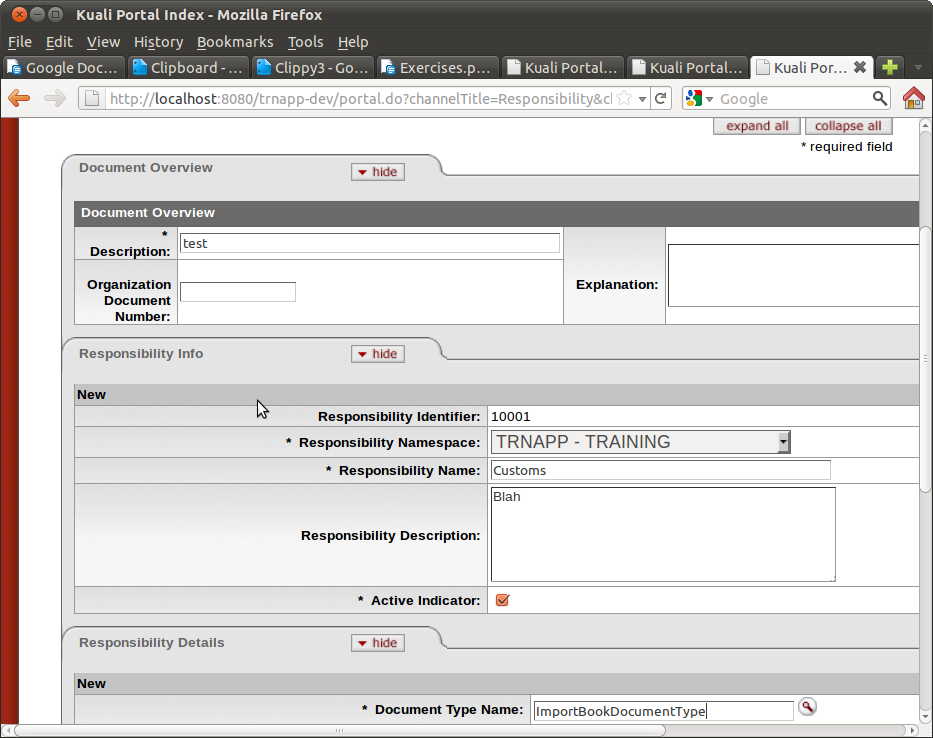
\includegraphics[width=\textwidth]{images/Screenshot21.png}

    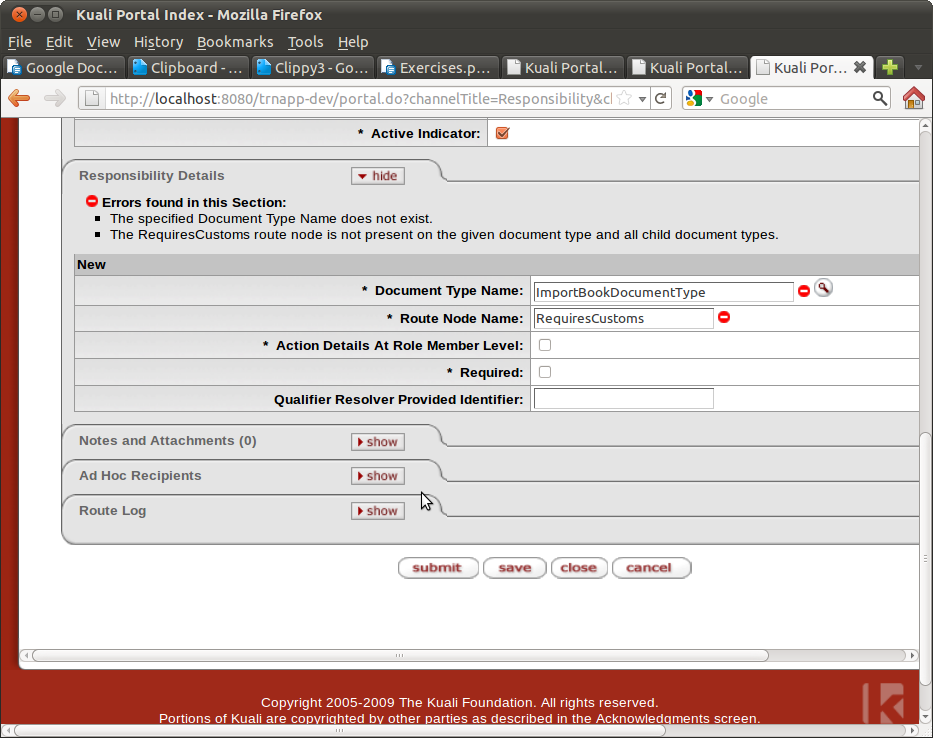
\includegraphics[width=\textwidth]{images/Screenshot22.png}
\end{enumerate}

\subsubsection*{2.2.2 Assign Customs Responsibility to the Customs Role}

\subsection*{2.3 Add a User to the Customs Role}

\subsection*{2.4 Update the ImportedBookOrderDocumentType.xml}
Now that the basic information has been created for the the derived
role, we need to tell Workflow to use it.

\begin{enumerate}
  \item Edit the \textbf{ImportedBookOrderDocumentType.xml}
  \item Add a \textbf{routePath}
\begin{lstlisting}[numbers=left,language=xml,basicstyle=\scriptsize,backgroundcolor=\color{ubergray},caption={ImportBookOrderDocument.xml},frame=single,breaklines=true]
   		 <routePaths>
   			 <routePath>
   				 <start name="AdHoc" nextNode="Warehouse Processing" />
   				 <role name="Warehouse Processing" nextNode="Customs" />
   				 <role name="Customs" />
   			 </routePath>
   		 </routePaths>
\end{lstlisting}
\item Add a \textbf{routeNode}
\begin{lstlisting}[numbers=left,language=xml,basicstyle=\scriptsize,backgroundcolor=\color{ubergray},caption={ImportBookOrderDocument.xml},frame=single,breaklines=true]
   		 <routeNodes>
   			 <start name="AdHoc" />
   			 <requests name="Warehouse Processing">
   				 <activationType>P</activationType>
   				 <ruleTemplate>WarehouseProcessingTemplate</ruleTemplate>
   			 </requests>
   			 <role name="Customs">
   				 <type>org.kuali.rice.kns.workflow.attribute.DataDictionaryQualifierResolver</type>
   			 </role>
   		 </routeNodes>
\end{lstlisting}
\end{enumerate}

\subsection*{2.5 Update the ImportedBookOrderDocument.xml}
\begin{lstlisting}[numbers=left,language=xml,basicstyle=\scriptsize,backgroundcolor=\color{ubergray},caption={ImportBookOrderDocument.xml},frame=single,breaklines=true]
	<bean
		id="DocumentValuePathGroup-ImportedBookOrderDocument-RequiresCustoms-bookOrderEntries"
		parent="org.kuali.rice.kns.workflow.attribute.DataDictionaryQualifierResolver">
		<property name="documentCollectionPath">
			<bean class="org.kuali.rice.kns.datadictionary.DocumentCollectionPath">
				<property name="collectionPath"
                value="bookOrderEntries" />
            </bean>
        </property>
     </bean>

\end{lstlisting}

\addcontentsline{toc}{subsection}{3 Complex Split Nodes}
\subsection*{3 Complex Split Nodes}

\subsection*{3.1 Modify the Existing ImportedBookOrderDocumentType.xml}

Now we edit the \textbf{ImportBookOrderDocumentType.xml} and add the
following \textbf{routePath} and \textbf{routeNode} information.
\begin{lstlisting}[numbers=left,language=xml,basicstyle=\scriptsize,backgroundcolor=\color{ubergray},caption={ImportBookOrderDocumentType.xml},frame=single,breaklines=true]
 <routePaths>
   			 <routePath>
   				 <start name="AdHoc" nextNode="Warehouse Processing" />
   				 <split name="RequiresCustoms"> 
                     <branch name="False">  
                     </branch> 
                     <branch name="True">
     				     <role name="Warehouse Processing" nextNode="Customs" />
     				     <role name="Customs" />
   				     </branch> 
                     <join name="JoinRequiresCustoms" /> 
                 </split>
   			 </routePath>
  </routePaths>
   		 <routeNodes>
   			 <start name="AdHoc" />
   			 <split name="RequiresCustoms">
   				 <type>
   					 org.kuali.rice.kew.actions.SimpleBooleanSplitNode
   				 </type>
   			 </split>
   			 <requests name="Warehouse Processing">
   				 <activationType>P</activationType>
   				 <ruleTemplate>WarehouseProcessingTemplate</ruleTemplate>
   			 </requests>
   			 <join name="JoinRequiresCustoms" />
   			 <role name="Customs">
   				 <type>org.kuali.rice.kns.workflow.attribute.DataDictionaryQualifierResolver
   				 </type>
   			 </role>
         </routeNodes>
\end{lstlisting}

\subsection*{3.2 Modify the ImportedBookOrderDocument.java}
The following \textbf{answerSplitNodeQuestion()} method must be overridden in the \textbf{ImportedBookOrderDocument}
\begin{lstlisting}[numbers=left,language=java,basicstyle=\scriptsize,backgroundcolor=\color{ubergray},caption={New
  KIM Type},frame=single,breaklines=true]
    /**
     * @see org.kuali.kfs.sys.document.FinancialSystemTransactionalDocumentBase#answerSplitNodeQuestion(java.lang.String)
     */
    @Override
    public boolean answerSplitNodeQuestion(String nodeName) throws UnsupportedOperationException {
        if ("RequiresCustoms".equals(nodeName)) {
            if (getBookOrderEntries().size() > 1) {
                return true;
            }
            else {
                return false;
            }
        }
        throw new UnsupportedOperationException("No split node logic
        defined for split node "+nodeName+" on the Imported Book Order
        document");
    }
\end{lstlisting}


\newpage
  {\setlength{\baselineskip}%
           {0.0\baselineskip}
  \section*{Notes}
  \hrulefill \par}